% ============================================================================
% TEMPLATE TESI - CORSO DI STUDIO IN INFORMATICA
% ============================================================================
% GUIDA RAPIDA ALLA STESURA PER GLI STUDENTI:
% 0. NOTA DI CONTESTO SULLE PREFERENZE METODOLOGICHE:
%    - Questo template e le relative linee guida didattiche rispecchiano fedelmente le preferenze
%      scientifiche e didattiche del Prof. Jesús Cevallos (docente di Probabilità e Statistica per l'Informatica),
%      allineate alla sua materia e ai suoi standard di ricerca epistemica e quantitativa.
%    - ATTENZIONE: Altri docenti e relatori di altre aree dell'informatica potrebbero avere specifiche,
%      convenzioni o preferenze metodologiche differenti; è sempre indispensabile concordare
%      l'impostazione finale con il proprio relatore di tesi.
%
% 1. REGOLE FORMALI DI COPERTINA:
%    - NOMENCLATURA UFFICIALE: Scrivere SEMPRE "CORSO DI STUDIO" e MAI "Corso di Laurea"!
%    - NOME IN COPERTINA: Inserire UNICAMENTE il Nome e Cognome dello studente (e Matricola),
%      SENZA premettere la parola "Candidato", "Candidata" o "Tesi di Laurea di:".
%
% 2. METODOLOGIA DI LAVORO IN 6 FASI:
%    1) Definizione della domanda di ricerca (fase più lunga e difficile, vale almeno 6 su 10!).
%    2) Definizione degli esperimenti e delle metriche per rispondere alla domanda senza ambiguità.
%    3) Implementazione del codice (il codice è uno STRUMENTO EPISTEMICO per rispondere alla domanda,
%       non un prodotto commerciale fine a se stesso).
%    4) Sperimentazione (raccolta dati riproducibile).
%    5) Analisi critica dei risultati.
%    6) Scrittura della tesi (Cap 4 e 5 per primi, Cap 1 e Abstract per ultimi).
%    - GESTIONE DELL'ANSIA E FALLBACK: Fissa sempre scadenze con piani di riserva espliciti e brutali
%      (es. "Implementazione entro data X; fallback: uso libreria open-source e rimodulazione domanda").
%
% 3. ORDINE CRONOLOGICO RACCOMANDATO PER LA SCRITTURA:
%    - Non iniziare a scrivere la tesi dal Capitolo 1!
%    - PERCHÉ? Spesso si sprecano troppo tempo ed energie sull'introduzione prima di sapere
%      cosa si farà davvero, lasciando poco tempo per le parti importanti (codice e risultati)
%      e fallendo lo SCOPE (il perimetro/confine degli obiettivi effettivamente realizzabili).
%    - FASE 1: Appena completato il lavoro di tesi/tirocinio/programmazione,
%              scrivere subito i Capitoli 4 (Implementazione) e 5 (Risultati).
%              È il momento in cui dettagli tecnici, scelte di design, metriche
%              e grafici sono più nitidi e concreti.
%    - FASE 2: Scrivere il Capitolo 3 (Progettazione/Architettura del sistema)
%              e il Capitolo 2 (Background teorico e stato dell'arte).
%    - FASE 3: Scrivere il Capitolo 6 (Conclusioni e sviluppi futuri).
%    - FASE 4 (PER ULTIMO): Scrivere il Capitolo 1 (Introduzione) e il Sommario/
%              Abstract. Solo quando le conclusioni sono state tratte e il lavoro
%              è completamente definito si può introdurre l'opera con precisione.
%
% 3. REQUISITO BIBLIOGRAFICO FONDAMENTALE:
%    - La tesi DEVE includere ALMENO 20 CITAZIONI BIBLIOGRAFICHE autorevoli.
%    - Consultare il Capitolo 2 per la guida dettagliata su come citare.
%
% 4. ISTRUZIONI DI COMPILAZIONE (da terminale):
%    - Con latexmk (automatico, consigliato):
%        latexmk -pdf main.tex
%    - Con pdflatex + biber (sequenza manuale completa):
%        pdflatex main.tex
%        biber main
%        pdflatex main.tex
%        pdflatex main.tex
%    - Visualizzare il file PDF generato:
%        xdg-open main.pdf   (su Linux)
%        open main.pdf       (su macOS)
% ============================================================================

\documentclass[12pt, a4paper, oneside]{book}

% Per generazione PDF/A conforme ai requisiti di archiviazione accademica
\usepackage[a-2b]{pdfx}

% Pacchetti di base
\usepackage{caption}
\captionsetup[table]{skip=10pt, belowskip=-5pt}
\captionsetup[figure]{skip=10pt, belowskip=-5pt}

\usepackage[utf8]{inputenc}
\usepackage[T1]{fontenc}
\usepackage[italian]{babel}
\usepackage[left=2.5cm, right=2.5cm, top=3cm, bottom=3cm]{geometry}
\usepackage{indentfirst}
\usepackage{enumitem}
\setlist{itemsep=0pt, parsep=0pt, topsep=5pt}
\raggedbottom
\usepackage[skip=10pt]{parskip}

% Formattazione titoli dei capitoli
\usepackage{titlesec}
\titleformat{\chapter}[display]{\normalfont\huge\bfseries\raggedright}{Capitolo \thechapter}{10pt}{\Huge}
\titlespacing*{\chapter}{0pt}{0pt}{20pt}

% Pacchetti per grafica e matematica
\usepackage{graphicx}
\usepackage{amsmath}
\usepackage{amssymb}
\usepackage{float}

% Pacchetti per formattazione del testo
\usepackage{setspace}
\usepackage{ragged2e}
\usepackage{afterpage}
\usepackage[bottom]{footmisc}

% Pacchetti per tabelle professionali
\usepackage{tabularx}
\usepackage{array}
\usepackage{booktabs}
\usepackage[table]{xcolor}

% Pacchetti per listati di codice sorgente
\usepackage{listings}

\definecolor{codebg}{rgb}{0.96,0.96,0.96}
\definecolor{commentgreen}{rgb}{0.0,0.5,0.0}
\definecolor{keywordblue}{rgb}{0.0,0.0,0.85}
\definecolor{stringred}{rgb}{0.7,0.1,0.1}

\lstdefinestyle{codestyle}{
    backgroundcolor=\color{codebg},
    commentstyle=\color{commentgreen}\itshape, 
    keywordstyle=\color{keywordblue}\bfseries, 
    stringstyle=\color{stringred},
    numberstyle=\tiny\color{gray},      
    basicstyle=\ttfamily\small,         
    breakatwhitespace=false,         
    breaklines=true,
    captionpos=t,
    keepspaces=true,                 
    numbers=left,
    numbersep=10pt,                  
    showspaces=false,                
    showstringspaces=false,
    showtabs=false,                  
    tabsize=4,
    frame=single,
    rulecolor=\color{lightgray}
}
\lstset{style=codestyle}
\renewcommand{\lstlistingname}{Codice}
\renewcommand{\lstlistlistingname}{Elenco dei codici}

% Pacchetti per la scrittura di pseudocodice e algoritmi formali
\usepackage{algorithm}
\usepackage{algpseudocode}
\floatname{algorithm}{Algoritmo}
\renewcommand{\algorithmicrequire}{\textbf{Dati in ingresso (Input):}}
\renewcommand{\algorithmicensure}{\textbf{Dati in uscita (Output):}}

% Pacchetti per collegamenti ipertestuali e riferimenti intelligenti
\usepackage{hyperref}
\hypersetup{
    colorlinks=true,
    linkcolor=black,
    citecolor=blue!70!black,
    urlcolor=blue!70!black
}
\usepackage{cleveref}

% Configurazione cleveref in italiano
\crefname{figure}{Fig.}{Fig.}
\Crefname{figure}{Figura}{Figure}
\crefname{table}{Tab.}{Tab.}
\Crefname{table}{Tabella}{Tabelle}
\crefname{equation}{Eq.}{Eq.}
\Crefname{equation}{Equazione}{Equazioni}
\crefname{listing}{Codice}{Codici}
\Crefname{listing}{Codice}{Codici}
\crefname{algorithm}{Alg.}{Alg.}
\Crefname{algorithm}{Algoritmo}{Algoritmi}
\crefname{chapter}{Cap.}{Cap.}
\Crefname{chapter}{Capitolo}{Capitoli}
\crefname{section}{Sez.}{Sez.}
\Crefname{section}{Sezione}{Sezioni}
\newcommand{\crefrangeconjunction}{, }

% Profondità dell'indice
\setcounter{tocdepth}{3}
\setcounter{secnumdepth}{3}

% Nuovi tipi di colonna centrata per tabelle tabularx
\newcolumntype{C}{>{\centering\arraybackslash}X}

% Configurazione intestazioni e numeri di pagina al centro in basso
\usepackage{fancyhdr}
\pagestyle{fancy}
\fancyhf{}
\fancyfoot[C]{\thepage}
\renewcommand{\headrulewidth}{0pt}

% Spaziature figure e tabelle nel testo
\setlength{\intextsep}{20pt}
\setlength{\textfloatsep}{20pt}

% Gestione bibliografia con BibLaTeX e Biber
\usepackage[autostyle]{csquotes} 
\usepackage[style=numeric,sorting=none,backend=biber]{biblatex}
\addbibresource{biblio.bib}

% Cartella immagini predefinita
\graphicspath{{img/}}

% Interlinea 1.5 come da standard di ateneo
\setstretch{1.5}
\renewcommand{\contentsname}{Indice}
\addto\captionsitalian{\renewcommand{\figurename}{Figura}}
\addto\captionsitalian{\renewcommand{\tablename}{Tabella}}

% ============================================================================
% INIZIO DOCUMENTO
% ============================================================================
\begin{document}

% ----------------------------------------------------------------------------
% FRONTESPIZIO (ANONIMIZZATO)
% ----------------------------------------------------------------------------
\hypersetup{pageanchor=false}
\thispagestyle{empty}
\begin{titlepage}
    \begin{center}
        \vspace{0.5cm}
    
        {\large \textbf{UNIVERSITÀ DEGLI STUDI DELL'INSUBRIA}} \\
        {\large \textbf{DIPARTIMENTO DI SCIENZE TEORICHE ED APPLICATE}} \\
        
        \vspace{0.8cm}
        
        % ATTENZIONE: Usare SEMPRE "CORSO DI STUDIO" e MAI "Corso di Laurea"!
        {\large CORSO DI STUDIO IN INFORMATICA}
        
        \vspace{1.5cm}
    
        
\includegraphics[width=0.30\columnwidth]{img/logo_insu.jpeg}
        
        \vspace{1.2cm}
        
        {\LARGE \textbf{[TITOLO DELLA TESI:}}\\
        \vspace{0.3cm}
        {\LARGE \textbf{SOTTOTITOLO DESCRITTIVO DEL PROGETTO]}}
        
        \vspace{1.8cm}
        
        \begin{minipage}[t]{0.48\textwidth}
            \raggedright
            \textbf{Relatore:}\\
            Chiar.mo Prof. Nome Cognome\\[0.4cm]
            \textbf{Correlatore:} \textit{(opzionale)}\\
            Dott. Nome Cognome
        \end{minipage}
        \hfill
        \begin{minipage}[t]{0.48\textwidth}
            \raggedleft
            % ATTENZIONE: Inserire UNICAMENTE Nome, Cognome e Matricola.
            % NON usare la dicitura "Candidato", "Candidata" o "Tesi di Laurea di:".
            Nome Cognome\\[0.2cm]
            Matricola: 123456
        \end{minipage}
    
        \vfill
        \centering
        Anno Accademico 20XX/20XX
    \end{center}
\end{titlepage}
\hypersetup{pageanchor=true}

% Giustificazione del testo
\justifying

% ----------------------------------------------------------------------------
% MATERIALE PRELIMINARE (FRONTMATTER)
% ----------------------------------------------------------------------------
\frontmatter

% Abstract / Sommario
\chapter*{Sommario}
\markboth{Sommario}{Sommario}
\addcontentsline{toc}{chapter}{Sommario}

\begin{quote}
\textbf{Nota per lo studente:} Il sommario (o abstract) è una sintesi autonoma dell'intera tesi di lunghezza compresa tra le 200 e le 400 parole. 
Deve contenere in forma concisa:
\begin{enumerate}
    \item Il \textbf{contesto} e il \textbf{problema} affrontato;
    \item L'\textbf{obiettivo} del progetto e la motivazione;
    \item La \textbf{metodologia} e le tecnologie adottate;
    \item I \textbf{principali risultati} quantitativi e qualitativi ottenuti;
    \item Le \textbf{conclusioni} e il valore aggiunto del contributo.
\end{enumerate}
\textbf{Regola d'oro:} Scrivere il sommario per \textbf{ULTIMO}, solo dopo aver concluso e validato tutti i capitoli della tesi!
\end{quote}

[Inserire qui il testo del sommario in lingua italiana...]

\vspace{1.5cm}

\section*{Abstract}
\begin{quote}
\textbf{Note for the student:} English translation of the Italian summary. Essential for international indexing and bachelor's degree archiving.
\end{quote}

[Insert English abstract translation here...]

\cleardoublepage

% Ringraziamenti (opzionali)
\chapter*{Ringraziamenti}
\markboth{Ringraziamenti}{Ringraziamenti}
\addcontentsline{toc}{chapter}{Ringraziamenti}

\textit{(Sezione opzionale: riservata ai ringraziamenti a relatori, correlatori, docenti, colleghi di laboratorio, familiari e persone care che hanno supportato il percorso di studi e lo svolgimento della tesi.)}

[Inserire qui i ringraziamenti...]

\cleardoublepage

% Indici del documento
\tableofcontents
\newpage
\listoftables      % Indice delle tabelle
\newpage
\listoffigures     % Indice delle figure
\newpage
\lstlistoflistings % Indice dei listati di codice
\cleardoublepage

% ----------------------------------------------------------------------------
% CORPO PRINCIPALE (MAINMATTER)
% ----------------------------------------------------------------------------
\mainmatter
\setcounter{chapter}{0} 

% ============================================================================
% CAPITOLO 1 — INTRODUZIONE
% ============================================================================
\chapter{Introduzione}
\label{cap:introduzione}

% ----------------------------------------------------------------------------
% NOTA METODOLOGICA FONDAMENTALE SULLA STESURA
% ----------------------------------------------------------------------------
\vspace{-0.3cm}
\noindent\rule{\textwidth}{1.2pt}
\vspace{0.1cm}

\textbf{\large REGOLE DI STESURA PER LO STUDENTE — LEGGERE PRIMA DI SCRIVERE:}
\vspace{0.2cm}
\begin{enumerate}
    \item \textbf{SCRIVERE QUESTO CAPITOLO PER ULTIMO:} Non iniziare MAI la scrittura della tesi dall'Introduzione! L'Introduzione e il Sommario vanno redatti \textbf{solo alla fine}, dopo aver completato le Conclusioni (\Cref{cap:conclusioni}).
    \item \textbf{PERCHÉ? (TEMPO, ENERGIE E RISCHIO DI FALLIRE LO SCOPE):}
    \begin{itemize}
        \item \emph{Trappola del tempo e delle energie:} Molti studenti commettono l'errore di iniziare dall'introduzione, spendendo settimane a limare frasi generiche. Questo consuma le energie migliori e lascia poco tempo per le parti cruciali: l'architettura, la scrittura del codice, l'esecuzione dei test e l'analisi rigorosa dei dati.
        \item \emph{Cos'è lo SCOPE (perimetro del progetto)?} In informatica e nell'ingegneria del software, lo \textbf{scope} definisce i confini esatti del lavoro: cosa il sistema fa, cosa deliberatamente \textbf{non} fa, quali requisiti sono inclusi e quali vincoli sono fissati.
        \item \emph{Il rischio di fallire lo scope:} All'inizio del lavoro non puoi sapere con certezza cosa funzionerà, quali ostacoli tecnici incontrerai o dove arriverà effettivamente il codice. Se scrivi l'introduzione all'inizio, rischi di promettere obiettivi che non realizzerai o di sbagliare il perimetro (scope) del progetto. Scrivendola alla fine, l'introduzione fotograferà fedelmente ciò che hai realmente costruito e validato.
    \end{itemize}
    \item \textbf{ORDINE DI STESURA CONSIGLIATO:}
    \begin{itemize}
        \item \textbf{Fase 1:} Capitoli \ref{cap:Implementazione} (Implementazione) e \ref{cap:risultati} (Risultati/Validazione);
        \item \textbf{Fase 2:} Capitolo \ref{cap:sistema} (Progettazione) e Capitolo \ref{cap:background} (Background/Stato dell'Arte);
        \item \textbf{Fase 3:} Capitolo \ref{cap:conclusioni} (Conclusioni);
        \item \textbf{Fase 4 (Finale):} Capitolo \ref{cap:introduzione} (Introduzione) e Sommario/Abstract.
    \end{itemize}
    \item \textbf{ALLINEAMENTO METODOLOGICO (PROF. JESÚS CEVALLOS):}
    Questo template e le linee guida didattiche qui esposte rispecchiano fedelmente le preferenze scientifiche e metodologiche del \textbf{Prof.~Jesús Cevallos (docente di Probabilità e Statistica per l'Informatica)}, coerenti con la sua materia e con i suoi criteri di ricerca epistemica e statistica. 
    \textbf{Attenzione:} Altri docenti e relatori di altre aree dell'informatica potrebbero avere convenzioni, specifiche e preferenze metodologiche differenti. È sempre buona prassi concordare l'impostazione e la struttura della tesi con il proprio relatore di riferimento.
\end{enumerate}

\noindent\rule{\textwidth}{1.2pt}
\vspace{0.4cm}

L'introduzione è il biglietto da visita della tesi: deve catturare l'interesse della commissione e del lettore, inquadrare chiaramente il problema all'interno del panorama informatico moderno e chiarire senza ambiguità il valore del contributo scientifico o ingegneristico sviluppato.

Di seguito viene illustrata la suddivisione standard raccomandata per questo capitolo.


% ============================================================================
\section{Contesto e Motivazione}
\label{sec:contesto-motivazione}
% ============================================================================

\textbf{Cosa scrivere in questa sezione:}
\begin{itemize}
    \item \textbf{Inquadramento generale:} Descrivere il settore di riferimento (ad esempio: intelligenza artificiale, sicurezza informatica, sistemi distribuiti, ingegneria del software, Internet of Things).
    \item \textbf{Rilevanza applicativa o scientifica:} Spiegare perché questo ambito è cruciale oggi (esigenze industriali, aumento delle minacce, normative emergenti, requisiti di affidabilità).
    \item \textbf{Riferimenti bibliografici iniziali:} Già nell'introduzione è opportuno citare standard internazionali o articoli chiave per dare autorevolezza alle affermazioni (ad esempio: normative tecniche come CENELEC EN 50716~\cite{en50716} per il software critico o studi recenti sulla sicurezza informatica~\cite{soderi2023railway}).
\end{itemize}

\textit{Esempio di apertura:}\\
Nei moderni sistemi informatici distribuiti e cyber-fisici, la sicurezza e la trasparenza decisionale sono diventate requisiti imprescindibili. Come evidenziato dai recenti standard internazionali di settore~\cite{en50716, soderi2023railway}, non è più sufficiente che un algoritmo fornisca un risultato corretto: è necessario garantire che il processo di elaborazione sia verificabile, tracciabile e resiliente ad attacchi malevoli come i \emph{False Data Injection Attacks} (FDIA)~\cite{liu2009false}. In questo contesto si inserisce la presente tesi di laurea...


% ============================================================================
\section{Definizione del Problema, Ipotesi e Obiettivi}
\label{sec:problema-obiettivi}
% ============================================================================

\textbf{Guida per lo studente — Cos'è davvero una ``Tesi''?}
\begin{itemize}
    \item \textbf{La tesi come affermazione (o negazione) specifica:} 
    Stando alla definizione accademica e scientifica, una \emph{tesi} non è un semplice argomento o una rassegna generica, ma è una \textbf{proposizione specifica che viene dimostrata} attraverso il lavoro svolto. Può essere un'affermazione oppure una negazione.
    \begin{itemize}
        \item \emph{Esempio di affermazione specifica:} ``\emph{È possibile creare una libreria che esegua la migrazione di modelli da PyTorch a Rust senza incrementare la superficie di attacco del codice di oltre il 15\%, misurato in termini di Attack Success Rate (ASR) a fronte degli attacchi A, B e C.}''
        \item \emph{Esempio di negazione:} ``\emph{Non è possibile garantire la consistenza forte in questo protocollo distribuito mantenendo una latenza inferiore a $X$\,ms in presenza di partizioni di rete.}''
    \end{itemize}
    \item \textbf{Il valore della specificità:} Più l'affermazione è circoscritta, quantitativa e precisa, minore è il rischio che la tesi sia falsa, generica o non dimostrabile. La specificità è il principale alleato dello studente per consentire una dimostrazione rigorosa con dati sperimentali.
    \item \textbf{Tesi $\neq$ Titolo della tesi:} Attenzione a non confondere la tesi con il titolo del documento. Il titolo è spesso sintetico o tematico (es. ``\emph{Studio e sviluppo di un convertitore PyTorch-Rust}''); la \emph{tesi} è la specifica risposta scientifica/ingegneristica che il lavoro intende convalidare.
    \item \textbf{L'Ipotesi (la domanda di ricerca vale 6 su 10):}
    La tesi è sempre la risposta a un'ipotesi di partenza, ovvero a una domanda di ricerca (es. ``\emph{È possibile ottenere il risultato $X$ rispettando il vincolo $Y$?}''):
    \begin{quote}
    \textbf{Regola aurea:} Su una scala da 1 a 10, formulare la domanda corretta \textbf{vale almeno 6}. Una domanda formulata male vanifica mesi di programmazione.
    \end{quote}
    Per porre una domanda sensata, non banale e significativa, è indispensabile \textbf{fare ricerca preliminare, contaminarsi con la letteratura, capire cosa sta succedendo nello stato dell'arte} e individuare dove risiede il valore reale.
    \item \textbf{Fattibilità nei tempi e con le risorse:} La domanda di ricerca deve essere commisurata al perimetro di una tesi triennale: deve essere risolvibile con le risorse di calcolo a disposizione e nei tempi previsti, evitando quesiti irrealizzabili.
\end{itemize}

\vspace{0.3cm}
\textbf{Articolazione concreta degli obiettivi nel testo della tesi:}
\begin{enumerate}
    \item \textbf{Domanda di ricerca (Research Question):} Formulare chiaramente l'interrogativo fondamentale;
    \item \textbf{Tesi sostenuta:} Esplicitare l'affermazione specifica che il lavoro intende dimostrare;
    \item \textbf{Obiettivi specifici (bullet points):} Elencare i passi ingegneristici concreti per dimostrarla:
    \begin{enumerate}
        \item Studio dello stato dell'arte e analisi dei requisiti formali;
        \item Progettazione dell'architettura software modulare;
        \item Implementazione del prototipo in linguaggio Python/C++/Rust;
        \item Definizione del piano sperimentale e delle metriche di validazione;
        \item Analisi critica dei risultati ottenuti e verifica dell'ipotesi iniziale.
    \end{enumerate}
\end{enumerate}


% ============================================================================
\section{Metodologia, Fasi del Lavoro e Gestione dei Fallback}
\label{sec:metodologia}
% ============================================================================

\textbf{Guida per lo studente — Il Ruolo del Codice e il Metodo di Lavoro:}

\subsection*{Il codice come strumento epistemico (non come prodotto fine a se stesso)}
Una domanda classica degli studenti è: \emph{<<Quanto peso date al codice o ai risultati rispetto al testo della tesi?>>}.
La risposta fondamentale è:
\begin{quote}
Il codice è importante unicamente perché ci permette di \textbf{rispondere alla domanda di ricerca con sicurezza e con zero ambiguità}. 
È uno \textbf{strumento epistemico} (uno strumento per produrre conoscenza e verità scientifica), \textbf{NON} un prodotto di ingegneria commerciale fine a se stesso.
\end{quote}
In questo senso, il peso del codice e dei risultati è già interamente racchiuso in quel \textbf{``6 su 10''} assegnato alla formulazione della domanda! Non occorre ostinarsi a riscrivere da zero architetture titaniche: è molto più efficace prendere gli strumenti e i framework esistenti, comprendere cosa permettono di fare e capire quale domanda significativa possiamo indagare e quale esperimento è realmente fattibile con ciò che abbiamo a disposizione.

\subsection*{La pipeline di lavoro in 6 fasi}
Il percorso corretto per realizzare la tesi si articola in sei fasi sequenziali:
\begin{enumerate}
    \item \textbf{Definizione della domanda di ricerca:} È la fase \textbf{più lunga e più difficile} dell'intero percorso, ed è fisiologico che lo sia. Non allarmarti se richiede tempo e fatica: una volta trovata la domanda giusta, le fasi successive sono già ampiamente instradate e il lavoro diventa molto più meccanico;
    \item \textbf{Definizione degli esperimenti e delle metriche:} Stabilire con precisione quali test eseguire e quali parametri misurare per rispondere alla domanda senza ambiguità;
    \item \textbf{Implementazione:} Scrivere il codice strettamente necessario per condurre gli esperimenti;
    \item \textbf{Sperimentazione:} Eseguire i test e raccogliere i log e i dati in modo riproducibile;
    \item \textbf{Analisi dei risultati:} Interpretare criticamente i dati raccolti;
    \item \textbf{Scrittura della tesi:} Redigere il documento (ricordando di scrivere prima i Capitoli \ref{cap:Implementazione} e \ref{cap:risultati}, e l'Introduzione per ultima).
\end{enumerate}

\subsection*{Gestione dell'ansia: scadenze e piani di Fallback}
La redazione di una tesi può generare ansia da prestazione o timore di non farcela entro i tempi di laurea. La strategia ingegneristica per neutralizzare l'ansia è la \textbf{pianificazione con fallback espliciti (anche brutali)}:
\begin{itemize}
    \item Fissa scadenze precise per ciascuna fase;
    \item Associa a ciascuna scadenza un piano di riserva categorico. 
    \item \emph{Esempio pratico:} \textbf{<<Implementazione dell'algoritmo proprietario entro il giorno $X$; se entro tale data il codice non converge, FALLBACK: si adotta la libreria open-source esistente e si adatta la domanda di ricerca alla valutazione comparativa delle prestazioni.>>}
\end{itemize}
Avere sempre un fallback prefissato toglie la paura del fallimento: qualunque imprevisto si verifichi, il percorso verso la conclusione della tesi è già tracciato e protetto.


% ============================================================================
\section{Struttura del Documento}
\label{sec:struttura-tesi}
% ============================================================================

La sezione conclusiva dell'introduzione descrive sinteticamente l'organizzazione del documento, fornendo una guida alla lettura per capitoli mediante riferimenti incrociati con il comando \texttt{\textbackslash Cref\{\dots\}}:

\begin{itemize}
    \item \textbf{\Cref{cap:background} --- Stato dell'arte e background teorico:} Introduce i fondamenti teorici del dominio affrontato, esamina le soluzioni presenti in letteratura e illustra le regole rigorose per la gestione delle citazioni bibliografiche (con il vincolo di inserire almeno 20 fonti autorevoli).
    \item \textbf{\Cref{cap:sistema} --- Progettazione del sistema:} Presenta l'analisi dei requisiti, l'architettura generale del sistema software e il modello matematico/concettuale alla base delle decisioni.
    \item \textbf{\Cref{cap:Implementazione} --- Implementazione:} Descrive le tecnologie adottate, l'ambiente di sviluppo, la struttura modulare del codice e le scelte ingegneristiche più significative.
    \item \textbf{\Cref{cap:risultati} --- Validazione e risultati sperimentali:} Espone la metodologia di test, le metriche quantitative adottate, i grafici sperimentali e la discussione critica dei dati raccolti.
    \item \textbf{\Cref{cap:conclusioni} --- Conclusioni e sviluppi futuri:} Riassume i risultati conseguiti, evidenzia i limiti riscontrati nella soluzione e propone future direzioni di ricerca ed evoluzione.
\end{itemize}
% ============================================================================
% CAPITOLO 2 — STATO DELL'ARTE E BACKGROUND TEORICO
% ============================================================================
\chapter{Stato dell'arte e background teorico}
\label{cap:background}

Questo capitolo introduce i fondamenti concettuali e tecnologici su cui poggia l'intero lavoro di tesi. 

\textbf{Perché la ricerca bibliografica è cruciale?} Studiare la letteratura e analizzare lo stato dell'arte non serve a fare un mero riassunto nozionistico, ma ha uno scopo scientifico fondamentale: \textbf{contaminarsi con i lavori esistenti per capire cosa sta succedendo davvero e formulare la domanda di ricerca corretta}. Ricorda che, su una scala da 1 a 10, la formulazione della domanda giusta \textbf{vale almeno 6}! Una domanda ben posta, specifica e misurabile è il presupposto indispensabile per costruire una tesi solida e fattibile nei tempi a disposizione.

Inoltre, questo capitolo contiene la \textbf{guida operativa dettagliata su come effettuare le citazioni bibliografiche in LaTeX}, specificando i criteri di qualità e le regole formali da rispettare.


% ============================================================================
\section{Guida Operativa alle Citazioni Bibliografiche}
\label{sec:guida-citazioni}
% ============================================================================

\noindent\fbox{
\parbox{0.96\textwidth}{
\textbf{\large REQUISITO OBBLIGATORIO DELLA TESI: ALMENO 20 CITAZIONI}
\vspace{0.2cm}\\
Ogni tesi di laurea in Informatica deve contenere un apparato bibliografico solido e professionale, composto da \textbf{non meno di 20 fonti bibliografiche autorevoli}. Non sono ammesse bibliografie superficiali o costituite prevalentemente da pagine web temporanee.
}
}
\vspace{0.4cm}

\subsection{Criteri di autorevolezza delle fonti}
Non tutte le fonti hanno lo stesso valore scientifico. Gli studenti devono seguire questa gerarchia di autorevolezza:
\begin{enumerate}
    \item \textbf{Articoli in riviste scientifiche peer-reviewed (\texttt{@article}):} Sono le fonti a più alto rigore accademico (ad es. IEEE Transactions, ACM Journals, Nature, Springer, Elsevier). Esempio di articolo citato nel testo: Friston~\cite{friston2010free} o Doshi-Velez e Kim~\cite{doshi2017towards}.
    \item \textbf{Atti di conferenze internazionali (\texttt{@inproceedings}):} In informatica, le migliori conferenze (IEEE S\&P, ACM CCS, USENIX, NeurIPS, ICSE) hanno tassi di accettazione molto selettivi e rappresentano lo stato dell'arte avanzato (ad es. Liu et al.~\cite{liu2009false}).
    \item \textbf{Libri di testo accademici e monografie (\texttt{@book}):} Ideali per definizioni formali, algoritmi consolidati e teoremi fondamentali (ad es. Ammann e Offutt~\cite{ammann2016introduction}, Parr et al.~\cite{parr2022active}).
    \item \textbf{Standard tecnici e normative (\texttt{@techreport}):} Documenti ufficiali emessi da organismi di standardizzazione internazionali come CENELEC, ISO, IEC, IEEE o RFC dell'IETF (ad es. EN 50716~\cite{en50716} ed EN 50128~\cite{en50128}).
    \item \textbf{Repository software e documentazione ufficiale (\texttt{@misc}):} Da usare con parsimonia per strumenti specifici utilizzati nel progetto, citando sempre l'autore o l'organizzazione e la data di accesso (ad es. Streamlit~\cite{streamlit2019}, Weights \& Biases~\cite{wandb2020}).
    \item \textbf{DA EVITARE come fonti primarie:} Wikipedia, blog personali, forum (StackOverflow), post su Medium o siti commerciali privi di revisione paritaria.
\end{enumerate}

\subsection{Comandi BibLaTeX per citare nel testo}
In questo template la bibliografia è gestita tramite il pacchetto \texttt{biblatex} con backend \texttt{biber}. I comandi principali a disposizione sono:

\begin{itemize}
    \item \texttt{\textbackslash cite\{chiave\}}: Inserisce il numero della citazione tra parentesi quadre.
    \begin{itemize}
        \item \textit{Sintassi:} \texttt{Come dimostrato in letteratura\textbackslash cite\{nidhra2012black\}.}
        \item \textit{Risultato:} Come dimostrato in letteratura~\cite{nidhra2012black}.
    \end{itemize}
    \item \texttt{\textbackslash textcite\{chiave\}}: Cita l'autore integrando il nome nel discorso corrente, seguito dal numero di citazione.
    \begin{itemize}
        \item \textit{Sintassi:} \texttt{\textbackslash textcite\{gunning2019xai\} presentano il programma XAI della DARPA.}
        \item \textit{Risultato:} \textcite{gunning2019xai} presentano il programma XAI della DARPA.
    \end{itemize}
    \item \texttt{\textbackslash cite[opzioni]\{chiave\}}: Permette di specificare numeri di pagina, capitoli o teoremi specifici della fonte.
    \begin{itemize}
        \item \textit{Sintassi:} \texttt{\textbackslash cite[p.~45]\{ammann2016introduction\}}
        \item \textit{Risultato:} \cite[p.~45]{ammann2016introduction}
    \end{itemize}
    \item \textbf{Citazioni multiple:} Si inseriscono le chiavi separate da virgola all'interno dello stesso comando:
    \begin{itemize}
        \item \textit{Sintassi:} \texttt{\textbackslash cite\{liu2009false, teixeira2015secure, deng2017false\}}
        \item \textit{Risultato:} \cite{liu2009false, teixeira2015secure, deng2017false}.
    \end{itemize}
\end{itemize}

\subsection{Regole sintattiche del file \texttt{biblio.bib}}
Nel file \texttt{biblio.bib} ogni voce bibliografica ha una struttura ben definita. Tre regole fondamentali:
\begin{enumerate}
    \item \textbf{Nomi degli autori:} Usare sempre il formato \texttt{Cognome, Nome} e separare più autori con la parola chiave \texttt{and}. Esempio:
\begin{lstlisting}[language=TeX]
author = {Ammann, Paul and Offutt, Jeff}
\end{lstlisting}
    \item \textbf{Preservare maiuscole e acronimi:} BibLaTeX può convertire i titoli in minuscolo secondo lo stile tipografico. Per preservare acronimi (es. FDIA, AI, TCP/IP) o nomi propri nel titolo, racchiuderli tra parentesi graffe:
\begin{lstlisting}[language=TeX]
title = {Attacchi {FDIA} in Reti {TCP/IP} Basate su {Linux}}
\end{lstlisting}
    \item \textbf{Identificatori digitali (DOI):} Quando un articolo dispone di un Digital Object Identifier (DOI), inserirlo sempre nel campo \texttt{doi = \{...\}}.
\end{enumerate}


% ============================================================================
\section{Fondamenti Teorici: Approccio Black-Box vs White-Box}
\label{sec:black-white}
% ============================================================================

\textbf{Guida per lo studente:} In questa sezione si presentano i concetti teorici fondamentali necessari a comprendere il problema. Nell'esempio della presente tesi, si confrontano i paradigmi di collaudo e validazione software.

Un approccio \emph{black-box} considera il sistema software come una scatola chiusa: si osservano esclusivamente gli ingressi e le uscite, misurando la corrispondenza tra il comportamento osservato e quello atteso~\cite{gunning2019xai}. Le metriche standard di rilevamento (accuratezza, precisione, recall, F1-score) valutano unicamente le prestazioni esterne~\cite{powers2020evaluation}. Il limite strutturale della validazione black-box~\cite{ammann2016introduction} è che due sistemi che producono i medesimi output risultano indistinguibili, anche quando il processo logico interno differisce radicalmente.

Al contrario, un approccio \emph{white-box} apre la scatola: ogni variabile di stato e quantità intermedia che concorre alla decisione finale viene resa esplicita, registrata e formalmente verificata~\cite{nidhra2012black}. Come sottolineato nella letteratura sull'Intelligenza Artificiale Spiegabile (XAI)~\cite{doshi2017towards}, la validazione white-box è l'unica metodologia in grado di accertare se un sistema informatico opera correttamente per le motivazioni appropriate, e non per coincidenze statistiche o distorsioni nei dati di test.


% ============================================================================
\section{Analisi dello Stato dell'Arte e Lavori Correlati}
\label{sec:lavori-correlati}
% ============================================================================

\textbf{Guida per lo studente:} Questa sezione è dedicata al confronto critico con i lavori esistenti. Lo studente deve rispondere a domande quali:
\begin{itemize}
    \item Quali soluzioni sono state proposte in letteratura per problemi simili?
    \item Quali sono i punti di forza e i limiti delle tecnologie attuali?
    \item In che cosa la soluzione proposta in questa tesi si differenzia o apporta un miglioramento?
\end{itemize}

Ad esempio, nello studio della sicurezza nei sistemi cyber-fisici (CPS), gli attacchi di tipo \emph{False Data Injection} (FDIA) sono stati formalizzati inizialmente da \textcite{liu2009false} nel contesto delle reti di distribuzione elettrica. Successivamente, \textcite{teixeira2015secure} e \textcite{deng2017false} ne hanno esteso la modellazione matematica ai sistemi di controllo industriale a tempo continuo, evidenziando come attacchi stealthy possano eludere i tradizionali rilevatori basati su residui quadratici. L'applicazione di tali minacce al dominio ferroviario è stata ampiamente documentata da \textcite{soderi2023railway}.


% ============================================================================
\section{Modelli Teorici Avanzati: Active Inference}
\label{sec:active-inference-bg}
% ============================================================================

\textbf{Guida per lo studente:} Inserire qui eventuali formalismi matematici o paradigmi computazionali avanzati utilizzati nella tesi (es. reti neurali, teoria dei grafi, crittografia, modelli bayesiani).

L'Active Inference è un framework sviluppato nelle neuroscienze computazionali~\cite{friston2010free, parr2022active}, fondato sul principio che un agente intelligente minimizza una quantità formale nota come Free Energy~\cite{friston2017active}. Il modello unifica percezione e azione mediante l'aggiornamento bayesiano delle credenze (predictive coding~\cite{rao1999predictive, feldman2010attention}) e la minimizzazione dell'incertezza attesa (Expected Free Energy)~\cite{friston2015epistemic, da2020active, parr2019generalised, schwartenbeck2019computational, mirza2019introducing}.

La trattazione dei dettagli architetturali e ingegneristici derivati da questo impianto teorico è demandata al \Cref{cap:sistema}.
% ============================================================================
% CAPITOLO 3 — PROGETTAZIONE DEL SISTEMA
% ============================================================================
\chapter{Progettazione del sistema}
\label{cap:sistema}

Questo capitolo illustra la fase di analisi e progettazione architetturale del sistema proposto. Lo studente deve mostrare la capacità di trasformare i requisiti teorici in un'architettura software strutturata, modulare e formalmente definita.

Inoltre, questo capitolo fornisce gli esempi pratici per l'inserimento e il corretto riferimento incrociato di:
\begin{itemize}
    \item \textbf{Figure e diagrammi} (\Cref{sec:esempi-figure});
    \item \textbf{Tabelle tipografiche con il pacchetto \texttt{booktabs}} (\Cref{sec:esempi-tabelle});
    \item \textbf{Formule ed equazioni matematiche numerate} (\Cref{sec:esempi-equazioni}).
\end{itemize}


% ============================================================================
\section{Analisi dei Requisiti}
\label{sec:requisiti}
% ============================================================================

\textbf{Guida per lo studente:} Prima di presentare l'architettura, descrivere i requisiti del sistema separandoli chiaramente in:
\begin{enumerate}
    \item \textbf{Requisiti Funzionali (RF):} Quali operazioni e funzionalità specifiche il sistema deve eseguire (es. RF1: Rilevamento di valori anomali sui sensori; RF2: Calcolo del punteggio di confidenza in tempo reale; RF3: Generazione automatica dei log di audit).
    \item \textbf{Requisiti Non Funzionali (RNF):} Proprietà qualitative del sistema, quali:
    \begin{itemize}
        \item \emph{Prestazioni e latenza:} Tempo massimo consentito per elaborare un singolo campione di input (es. $< 100$\,ms);
        \item \emph{Trasparenza e tracciabilità (White-box):} Esposizione di tutte le variabili intermedie per consentire l'ispezione;
        \item \emph{Modularità ed estensibilità:} Facilità di sostituzione dei moduli interni o aggiunta di nuovi scenari di test;
        \item \emph{Riproducibilità:} Garanzia che a parità di seme casuale (\emph{random seed}) e configurazione, i risultati siano identici al 100\%.
    \end{itemize}
\end{enumerate}


% ============================================================================
\section{Architettura Generale del Sistema}
\label{sec:architettura-generale}
% ============================================================================

\textbf{Guida per lo studente:} Descrivere l'architettura complessiva ad alto livello, spiegando come i vari macro-componenti cooperano tra loro e qual è il flusso dei dati.


% ----------------------------------------------------------------------------
\subsection{Esempio di inserimento di figure in LaTeX}
\label{sec:esempi-figure}
% ----------------------------------------------------------------------------

Ogni figura inserita nella tesi deve:
\begin{enumerate}
    \item Essere racchiusa nell'ambiente \texttt{figure} con posizionatore (es. \texttt{[htbp]});
    \item Avere un file sorgente in formato vettoriale (PDF) o raster ad alta risoluzione (PNG, JPEG da almeno 300 DPI) memorizzato nella cartella \texttt{img/};
    \item Essere provvista di una didascalia esplicativa (\texttt{\textbackslash caption\{\dots\}});
    \item Avere un'etichetta univoca (\texttt{\textbackslash label\{fig:\dots\}}) posizionata \textbf{sempre dopo} il caption;
    \item \textbf{Essere sempre citata nel testo} con \texttt{\textbackslash Cref\{fig:\dots\}} o \texttt{\textbackslash ref\{fig:\dots\}}. Una figura mai citata nel testo è un grave errore metodologico.
\end{enumerate}

La \Cref{fig:architettura-esempio} illustra a titolo di esempio uno schema architetturale e di pipeline (sostituibile con il diagramma UML o architetturale specifico della tesi), evidenziando le fasi di acquisizione, pre-elaborazione, estrazione delle feature e classificazione/decisione.

\begin{figure}[htbp]
    \centering
    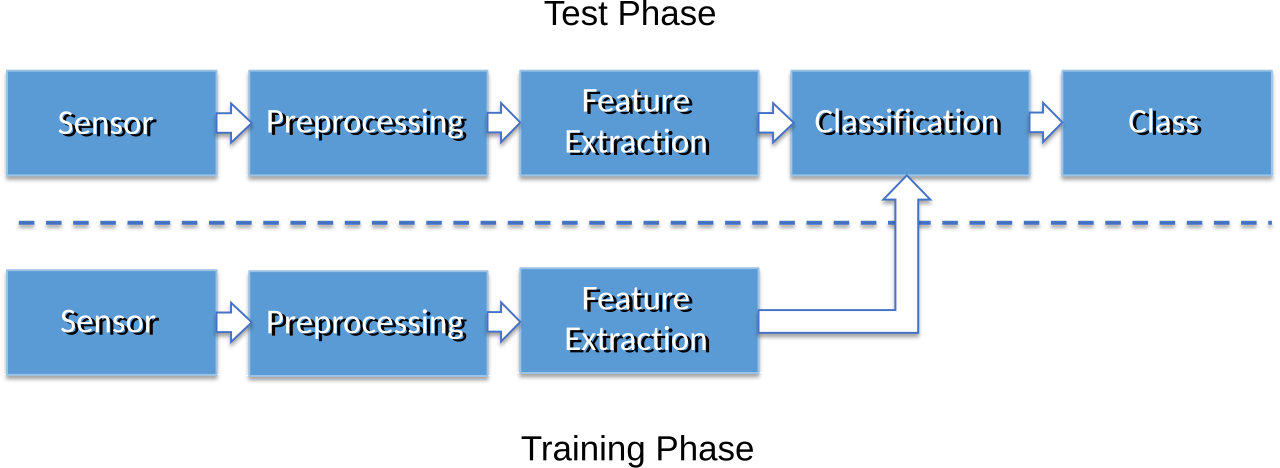
\includegraphics[width=0.92\textwidth]{placeholder_figura.png}
    \caption{Esempio di schema architetturale e pipeline di elaborazione a blocchi (ispirato allo standard di riconoscimento e classificazione, Wikimedia Commons). Nel lavoro di tesi, sostituire questa figura con l'architettura specifica del proprio sistema o software.}
    \label{fig:architettura-esempio}
\end{figure}

% ----------------------------------------------------------------------------
\subsection{Esempio di diagramma di flusso (Flowchart)}
\label{sec:esempi-flowchart}
% ----------------------------------------------------------------------------

Accanto ai diagrammi architetturali (che mostrano la struttura statica dei moduli o delle pipeline), i \textbf{diagrammi di flusso (flowchart)} sono fondamentali per rappresentare visivamente la dinamica temporale, le diramazioni condizionali (\texttt{if-else}) e la sequenza delle operazioni decisionali. 

Un diagramma di flusso chiaro ed elegante \textbf{sostituisce con enorme efficacia lunghe pagine di codice sorgente}: permette al docente e alla commissione di cogliere la logica algoritmica in pochi istanti, senza perdersi nei dettagli implementativi di basso livello.

La \Cref{fig:diagramma-flusso} riporta un classico diagramma di flusso a norma ISO, illustrando l'uso standard dei blocchi di inizio/fine (ovali), di controllo condizionale (rombi di decisione con rami \textit{Yes/No}) e di elaborazione/azione (rettangoli).

\begin{figure}[htbp]
    \centering
    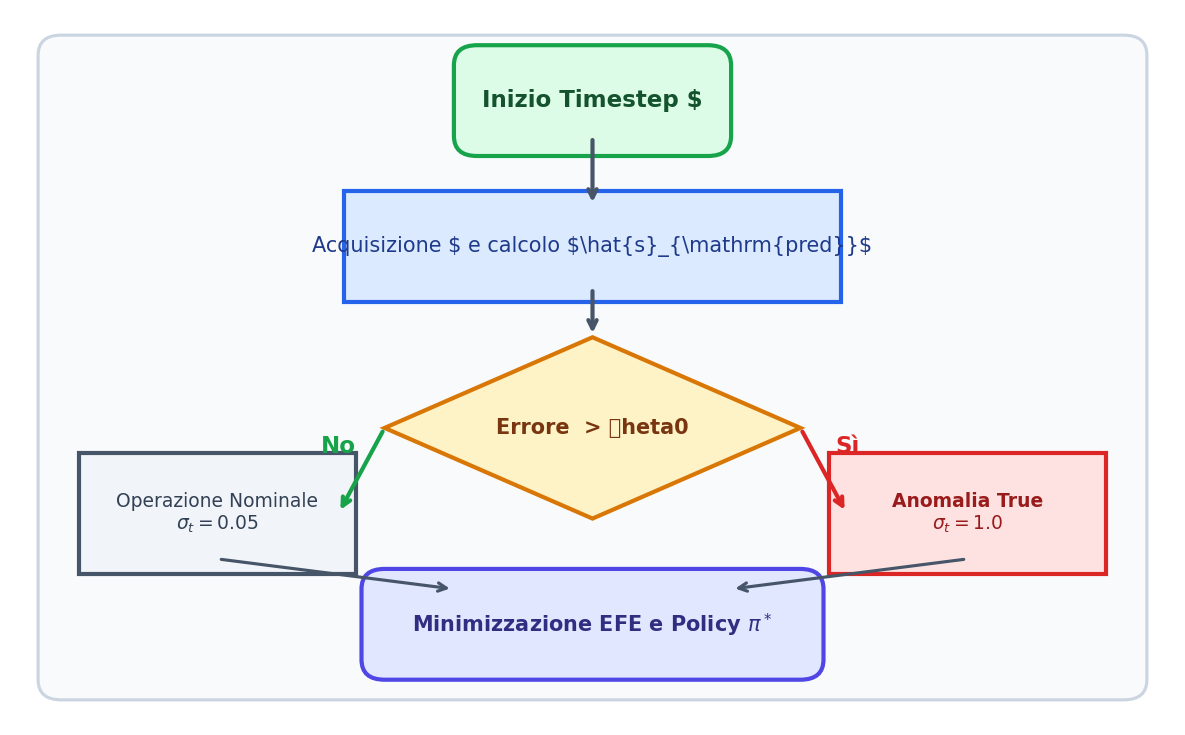
\includegraphics[width=0.45\textwidth]{placeholder_flusso.png}
    \caption{Esempio canonico di diagramma di flusso decisionale conforme agli standard grafici di processo (Wikimedia Commons). Nella tesi, sostituire con il flusso decisionale o computazionale del proprio algoritmo.}
    \label{fig:diagramma-flusso}
\end{figure}


% ============================================================================
\section{Componenti e Moduli Software}
\label{sec:moduli-sistema}
% ============================================================================

\textbf{Guida per lo studente:} Descrivere i singoli moduli software del sistema, le loro responsabilità e le interfacce esposte. Nel contesto del progetto di tesi, i componenti principali sono:

\begin{itemize}
    \item \textbf{Modulo Ambiente e Sensori (\texttt{Environment}):} Modella la dinamica fisica e lo strato sensoriale, introducendo rumore gaussiano o simulando iniezioni di dati malevoli;
    \item \textbf{Modello Generativo Interno (\texttt{GenerativeModel}):} Codifica la conoscenza a priori del sistema e genera predizioni sullo stato atteso;
    \item \textbf{Modulo di Stima dello Stato (\texttt{BeliefState}):} Calcola l'errore di predizione tra valore osservato e valore previsto, aggiornando la stima di incertezza posteriore;
    \item \textbf{Controllore Decisionale (\texttt{Controller}):} Valuta lo spazio delle azioni possibili attraverso una funzione di costo formale ed emette il comando attuativo.
\end{itemize}


% ----------------------------------------------------------------------------
\subsection{Linee guida ed esempio per la composizione di tabelle scientifiche}
\label{sec:esempi-tabelle}
% ----------------------------------------------------------------------------

Nelle pubblicazioni scientifiche e nelle tesi di laurea in Informatica, le tabelle devono rispettare precisi canoni tipografici:
\begin{enumerate}
    \item \textbf{Nessuna linea verticale:} Non usare mai linee verticali (\texttt{|}); rendono la lettura pesante e disordinata;
    \item \textbf{Pacchetto \texttt{booktabs}:} Usare esclusivamente le tre linee orizzontali ad alto valore tipografico: \texttt{\textbackslash toprule} (inizio), \texttt{\textbackslash midrule} (separatore intestazione) e \texttt{\textbackslash bottomrule} (chiusura);
    \item \textbf{Allineamento:} Allineare a sinistra (\texttt{l}) i testi descrittivi, al centro (\texttt{c}) i codici o stati, e a destra (\texttt{r}) i valori numerici;
    \item \textbf{Unità di misura nell'intestazione:} Inserire sempre l'unità di misura (es. ms, km/h, \%) nell'intestazione della colonna, mai ripetuta in ogni singola cella;
    \item \textbf{Didascalia e posizionamento:} La didascalia (\texttt{\textbackslash caption}) va posizionata preferibilmente \textbf{in alto} per le tabelle, seguita subito dal comando \texttt{\textbackslash label\{tab:\dots\}};
    \item \textbf{Riferimento obbligatorio:} Ogni tabella deve essere citata nel testo con \texttt{\textbackslash Cref\{tab:\dots\}}.
\end{enumerate}

La \Cref{tab:parametri-esempio} mostra una tabella tipografica standard compilata secondo queste direttive.

\begin{table}[htbp]
\centering
\small
\caption{Parametri di configurazione del sistema software.}
\label{tab:parametri-esempio}
\renewcommand{\arraystretch}{1.3}
\begin{tabular}{l c r l}
\toprule
\textbf{Parametro} & \textbf{Tipo} & \textbf{Default} & \textbf{Descrizione} \\
\midrule
\texttt{NUM\_STEPS}          & Intero  & 50    & Durata temporale della simulazione (passi) \\
\texttt{SENSOR\_NOISE}       & Float   & 0.05  & Ampiezza del rumore additivo uniforme ($\pm$) \\
\texttt{ANOMALY\_THRESHOLD}  & Float   & 0.30  & Soglia sul prediction error per anomalia \\
\texttt{DEFAULT\_SPEED}      & Float   & 10.0  & Velocità di marcia nominale (km/h) \\
\texttt{REDUCED\_SPEED}      & Float   & 4.0   & Velocità cautelativa con alta incertezza (km/h) \\
\texttt{STOP\_SPEED}         & Float   & 0.0   & Velocità di arresto immediato (km/h) \\
\bottomrule
\end{tabular}
\end{table}


% ============================================================================
\section{Modello Matematico e Logica Decisionale}
\label{sec:modello-matematico}
% ============================================================================

\textbf{Guida per lo studente:} Se la tesi impiega modelli probabilistici, equazioni differenziali, formule di costo o funzioni obiettivo, formalizzarli con precisione matematica.


% ----------------------------------------------------------------------------
\subsection{Esempio di inserimento di equazioni matematiche}
\label{sec:esempi-equazioni}
% ----------------------------------------------------------------------------

Le equazioni matematiche importanti devono essere posizionate nell'ambiente \texttt{equation}, dotate di etichetta \texttt{\textbackslash label\{eq:\dots\}} e referenziate con \texttt{\textbackslash Cref\{eq:\dots\}}.

Ad esempio, l'errore di predizione sensoriale $e_t$ al tempo $t$ è calcolato come discrepanza assoluta tra l'osservazione $o_t$ e la predizione $\hat{s}_t$:
\begin{equation}
e_t = \left| o_t - \hat{s}_t \right|
\label{eq:prediction-error}
\end{equation}

Quando l'errore di predizione $e_t$ definito nell'\Cref{eq:prediction-error} eccede la soglia $\theta_{\mathrm{anomalia}}$, il livello di incertezza $\sigma_t$ viene elevato al valore massimo.

La selezione della politica decisionale ottima $\pi^*$ avviene minimizzando la funzione obiettivo di Expected Free Energy (EFE), composta da una componente pragmatica e da una componente epistemica~\cite{friston2015epistemic}:
\begin{equation}
\pi^* = \arg\min_{\pi} \left[ -\mathrm{PragmaticValue}(\pi) - \mathrm{EpistemicValue}(\pi) \right]
\label{eq:efe-decision}
\end{equation}


% ----------------------------------------------------------------------------
\subsection{Esempio di inserimento di algoritmi in pseudocodice formale}
\label{sec:esempi-algoritmi}
% ----------------------------------------------------------------------------

Quando si descrive un procedimento computazionale in modo indipendente dallo specifico linguaggio di programmazione, è preferibile utilizzare lo **pseudocodice formale** tramite i pacchetti \texttt{algorithm} e \texttt{algpseudocode}.

I comandi principali dell'ambiente \texttt{algorithmic} sono:
\begin{itemize}
    \item \texttt{\textbackslash Require} e \texttt{\textbackslash Ensure}: Definiscono i dati in ingresso (input/precondizioni) e in uscita (output/postcondizioni);
    \item \texttt{\textbackslash State}: Introduce un'istruzione elementare o un'assegnazione ($\gets$ ottenuto con \texttt{\textbackslash gets});
    \item \texttt{\textbackslash If\{cond\} \dots \textbackslash Else \dots \textbackslash EndIf}: Blocchi condizionali;
    \item \texttt{\textbackslash For\{cond\} \dots \textbackslash EndFor} e \texttt{\textbackslash While\{cond\} \dots \textbackslash EndWhile}: Strutture iterative;
    \item \texttt{\textbackslash Call\{NomeFunzione\}\{Argomenti\}}: Invocazione di una procedura o metodo;
    \item \texttt{\textbackslash Comment\{testo\}}: Inserimento di commenti esplicativi a margine.
\end{itemize}

L'\Cref{alg:decision-process} illustra il ciclo di stima dello stato e decisione ottima eseguito a ogni passo temporale.

\begin{algorithm}[htbp]
\caption{Ciclo decisionale del controllore Active Inference.}
\label{alg:decision-process}
\begin{algorithmic}[1]
    \Require Osservazione sensoriale $o_t \in \mathbb{R}$, passo temporale $t \in \mathbb{N}$, soglia di anomalia $\theta \in \mathbb{R}^+$
    \Ensure Azione ottima selezionata $\pi^*$, credenza aggiornata $\hat{s}_t$
    \vspace{0.15cm}
    \State $\hat{s}_{\mathrm{pred}} \gets \Call{GenerativeModelPredict}{t}$ \Comment{Predizione dal prior interno}
    \State $e_t \gets |o_t - \hat{s}_{\mathrm{pred}}|$ \Comment{Calcolo del prediction error}
    \If{$e_t > \theta$}
        \State $\mathrm{anomalia} \gets \mathbf{True}$
        \State $\sigma_t \gets 1.0$ \Comment{Massima incertezza: sensore ritenuto inaffidabile}
        \State $\hat{s}_t \gets \hat{s}_{\mathrm{pred}}$ \Comment{L'agente si affida al modello generativo}
    \Else
        \State $\mathrm{anomalia} \gets \mathbf{False}$
        \State $\sigma_t \gets 0.05$ \Comment{Incertezza nominale (rumore di fondo)}
        \State $\hat{s}_t \gets o_t$ \Comment{L'agente acquisisce il dato dal sensore}
    \EndIf
    \For{\textbf{ciascuna} politica d'azione $\pi \in \Pi$}
        \State $\mathrm{val}_{\mathrm{pragmatic}} \gets \Call{ComputePragmaticValue}{\pi, \hat{s}_t}$
        \State $\mathrm{val}_{\mathrm{epistemic}} \gets \Call{ComputeEpistemicValue}{\pi, \sigma_t}$
        \State $\mathrm{EFE}(\pi) \gets -\mathrm{val}_{\mathrm{pragmatic}} - \mathrm{val}_{\mathrm{epistemic}}$
    \EndFor
    \State $\pi^* \gets \arg\min_{\pi \in \Pi} \mathrm{EFE}(\pi)$ \Comment{Selezione dell'azione che minimizza l'EFE}
    \State \Return $\pi^*, \hat{s}_t$
\end{algorithmic}
\end{algorithm}

Nel \Cref{cap:Implementazione} verrà esaminata l'implementazione concreta di tale algoritmo all'interno del codice Python sorgente.

% ============================================================================
% CAPITOLO 4 — IMPLEMENTAZIONE
% ============================================================================
\chapter{Implementazione}
\label{cap:Implementazione}

% ----------------------------------------------------------------------------
% NOTA METODOLOGICA FONDAMENTALE SULLA STESURA
% ----------------------------------------------------------------------------
\noindent\fbox{
\parbox{0.96\textwidth}{
\textbf{\large REGOLE DI STESURA PER LO STUDENTE — LEGGERE PRIMA DI SCRIVERE:}
\vspace{0.2cm}
\begin{enumerate}
    \item \textbf{QUESTO È IL PRIMO CAPITOLO DA SCRIVERE (INSIEME AL CAPITOLO 5):} Non appena hai completato il codice, il simulatore o il prototipo software della tesi, \textbf{inizia subito la scrittura da questo capitolo e dal \Cref{cap:risultati}}.
    \item \textbf{PERCHÉ?} L'architettura software, le librerie usate, le classi create, i bug risolti e i dettagli implementativi sono vivi nella tua memoria. Aspettare settimane prima di documentarli porta inevitabilmente a dimenticare motivazioni tecniche e dettagli critici.
    \item \textbf{DOPO AVER SCRITTO QUESTO CAPITOLO E IL CAPITOLO 5:} Passa al \Cref{cap:sistema} (Progettazione formale), poi al \Cref{cap:background} (Stato dell'arte), poi al \Cref{cap:conclusioni} (Conclusioni), e solo alla fine di tutto al \Cref{cap:introduzione} (Introduzione).
\end{enumerate}
}
}
\vspace{0.6cm}

Questo capitolo documenta la realizzazione pratica del software sviluppato nel lavoro di tesi. Lo scopo è spiegare come l'architettura concettuale definita nel \Cref{cap:sistema} è stata tradotta in codice funzionante, manutenibile e riproducibile.

\textbf{Nota epistemologica sul codice:} Il software sviluppato in una tesi di laurea non deve essere inteso come un prodotto commerciale fine a se stesso, bensì come uno \textbf{strumento epistemico} rigoroso: il suo valore risiede nell'eliminare ogni ambiguità e nel permettere di rispondere con precisione scientifica alla domanda di ricerca.

Inoltre, il capitolo contiene le indicazioni per inserire ed evidenziare porzioni di codice sorgente tramite il pacchetto \texttt{listings}.


% ============================================================================
\section{Ambiente di Sviluppo e Tecnologie Utilizzate}
\label{sec:ambiente-sviluppo}
% ============================================================================

\textbf{Guida per lo studente:} Riportare in questa sezione lo stack tecnologico completo, specificando:
\begin{itemize}
    \item \textbf{Linguaggio di programmazione e runtime:} Versione del linguaggio (es. Python 3.11+, C++20, Java 21 LTS) e relative motivazioni (es. determinismo, velocità di prototipazione, ecosistema scientifico);
    \item \textbf{Librerie e framework core:} Librerie matematiche (es. NumPy, SciPy), framework per GUI/Web (es. Streamlit~\cite{streamlit2019}, Flask, FastAPI) e strumenti di tracciamento degli esperimenti (es. Weights \& Biases~\cite{wandb2020});
    \item \textbf{Gestione dell'ambiente e dipendenze:} Specificare l'uso di ambienti virtuali (\texttt{venv}, \texttt{conda}) o container (\texttt{Docker}) per garantire la portabilità dell'applicazione;
    \item \textbf{Sistema di controllo versione:} Organizzazione del repository Git, suddivisione dei branch e convenzioni sui commit.
\end{itemize}


% ============================================================================
\section{Organizzazione del Repository e Struttura Modulare}
\label{sec:struttura-codice}
% ============================================================================

\textbf{Guida per lo studente:} Mostrare l'albero delle directory del progetto e spiegare la responsabilità assegnata a ciascun file sorgente.

Un esempio tipico di organizzazione del codice in un progetto di tesi in Informatica è il seguente:

\begin{itemize}
    \item \texttt{constants.py} --- Centralizza tutte le costanti di configurazione, i percorsi e le soglie numeriche, evitando valori \emph{hard-coded} sparsi nel codice;
    \item \texttt{environment.py} --- Implementa la simulazione dell'ambiente fisico e lo strato sensoriale;
    \item \texttt{belief\_state.py} --- Gestisce l'aggiornamento bayesiano dello stato interno e il rilevamento delle anomalie;
    \item \texttt{controller.py} --- Implementa il calcolo della funzione obiettivo e la selezione della decisione ottima;
    \item \texttt{simulation.py} --- Coordina il ciclo principale (\emph{main loop}) dell'esperimento ed esporta i log di tracciamento;
    \item \texttt{visualize.py} --- Genera i grafici statistici e le rappresentazioni grafiche utilizzate nel documento di tesi.
\end{itemize}


% ============================================================================
\section{Dettagli Implementativi e Listati di Codice}
\label{sec:dettagli-codice}
% ============================================================================

\textbf{Guida per lo studente:} Non riportare centinaia di righe di codice banale (come getter, setter o parser standard). Inserire unicamente gli snippet essenziali che contengono il cuore algoritmico della tesi.

Ogni listato di codice deve:
\begin{enumerate}
    \item Essere racchiuso nell'ambiente \texttt{\textbackslash begin\{lstlisting\}[language=\dots, caption=\dots, label=\dots]};
    \item Possedere una didascalia (\texttt{caption}) che descriva brevemente cosa realizza il codice;
    \item Avere un'etichetta (\texttt{label=\{lst:\dots\}}) per il riferimento incrociato;
    \item Essere accompagnato da una spiegazione puntuale nel testo che commenta la logica del codice linea per linea.
\end{enumerate}

Il \Cref{lst:belief-update} mostra la logica di calcolo dell'errore di predizione e dell'aggiornamento dell'incertezza implementata nel modulo \texttt{BeliefState}:

\begin{lstlisting}[language=Python, caption={Logica di aggiornamento percettivo nel \texttt{BeliefState}.}, label={lst:belief-update}]
def update(self, sensor_value: float, t: int) -> None:
    # 1. Calcolo del valore atteso dal modello interno
    expected_value = self.generative_model.predict(t)
    
    # 2. Calcolo del prediction error
    self.prediction_error = abs(sensor_value - expected_value)
    
    # 3. Confronto con la soglia di anomalia
    if self.prediction_error > self.anomaly_threshold:
        self.anomaly_detected = True
        self.uncertainty = 1.0          # Massima incertezza
        self.estimate = expected_value  # Priorita al modello interno
    else:
        self.anomaly_detected = False
        self.uncertainty = 0.1          # Livello base di rumore
        self.estimate = sensor_value    # Fiducia nel sensore
\end{lstlisting}

Come si può osservare nel \Cref{lst:belief-update}, quando il valore assoluto della differenza supera la soglia prefissata, l'incertezza sale immediatamente al valore massimo ($1.0$), innescando una risposta cautelativa nel controllore.


% ============================================================================
\section{Scelte Progettuali e Criticità Risolte}
\label{sec:scelte-criticita}
% ============================================================================

\textbf{Guida per lo studente:} Spiegare in modo onesto e analitico le sfide tecniche incontrate durante lo sviluppo e le soluzioni adottate:
\begin{itemize}
    \item \textbf{Scelte architetturali:} Perché è stato scelto un pattern rispetto a un altro (es. ereditarietà vs composizione, architettura a eventi vs polling sincrono)?
    \item \textbf{Efficienza computazionale:} Quali ottimizzazioni sono state necessarie per rispettare i requisiti temporali (es. vettorizzazione delle operazioni numeriche in NumPy)?
    \item \textbf{Gestione degli errori e robustezza:} Come sono state gestite eccezioni, valori nulli, timeout di rete o input sensoriali fuori scala?
\end{itemize}

L'analisi dei risultati prodotti dall'esecuzione di questo software è presentata in dettaglio nel successivo \Cref{cap:risultati}.
    
% ============================================================================
% CAPITOLO 5 — RISULTATI SPERIMENTALI E VALIDAZIONE
% ============================================================================
\chapter{Risultati e validazione}
\label{cap:risultati}

% ----------------------------------------------------------------------------
% NOTA METODOLOGICA FONDAMENTALE SULLA STESURA
% ----------------------------------------------------------------------------
\noindent\fbox{
\parbox{0.96\textwidth}{
\textbf{\large REGOLE DI STESURA PER LO STUDENTE — LEGGERE PRIMA DI SCRIVERE:}
\vspace{0.2cm}
\begin{enumerate}
    \item \textbf{SCRIVERE QUESTO CAPITOLO SUBITO DOPO IL CAPITOLO 4:} Non appena hai raccolto i dati dei test e generato i grafici, \textbf{redigi immediatamente questo capitolo}!
    \item \textbf{PERCHÉ?} I numeri, le configurazioni sperimentali, i parametri dei test e il significato delle anomalie osservate sono ancora chiari e verificabili. Se aspetti, rischi di dimenticare le condizioni esatte in cui sono stati eseguiti i test.
    \item \textbf{STRUTTURA SCIENTIFICA:} Un capitolo di risultati deve sempre seguire questo schema logico:
    \begin{itemize}
        \item Prima si definisce la \textbf{metodologia di test};
        \item Poi si definiscono formalmente le \textbf{metriche matematiche};
        \item Poi si mostrano i \textbf{dati quantitativi} (tabelle e grafici);
        \item Infine si conduce una \textbf{discussione critica} approfondita (senza limitarsi a descrivere i grafici).
    \end{itemize}
\end{enumerate}
}
}
\vspace{0.6cm}

Questo capitolo presenta la metodologia di validazione adottata e i risultati sperimentali ottenuti per verificare l'efficacia, la correttezza e la robustezza del sistema proposto.


% ============================================================================
\section{Metodologia di Validazione e Setup Sperimentale}
\label{sec:metodologia-validazione}
% ============================================================================

\textbf{Guida per lo studente:} Descrivere dettagliatamente l'ambiente e gli scenari in cui sono stati svolti i test per garantire la riproducibilità scientifica:
\begin{itemize}
    \item \textbf{Ambiente hardware e software di test:} Specifiche della macchina (CPU, RAM, OS, versione runtime);
    \item \textbf{Dataset o scenari di simulazione:} Descrizione dei dati utilizzati (dimensioni, provenienza, split train/test o parametri di generazione sintetica);
    \item \textbf{Scenari di test strutturati:}
    \begin{enumerate}
        \item \emph{Funzionamento nominale (Baseline):} Verifica del comportamento del sistema in condizioni ordinarie prive di disturbi;
        \item \emph{Analisi dei componenti (Ablation Study):} Rimozione selettiva di singoli moduli per verificare se ciascuno di essi è strettamente necessario;
        \item \emph{Stress Test e casi limite:} Valutazione del comportamento del sistema a fronte di input malformati, rumore estremo o attacchi malevoli coordinati.
    \end{enumerate}
\end{itemize}


% ============================================================================
\section{Definizione delle Metriche di Valutazione}
\label{sec:metriche-valutazione}
% ============================================================================

\textbf{Guida per lo studente:} Tutte le metriche utilizzate nelle tabelle e nei grafici devono essere definite formalmente \textbf{prima} di presentare i risultati numerici~\cite{powers2020evaluation}.

Nel caso di sistemi di rilevamento e classificazione, le metriche standard basate sulla matrice di confusione sono definite come segue:

\begin{itemize}
    \item \textbf{Precision (Precisione):} Frazione di allarmi generati che corrispondono a reali anomalie:
    \begin{equation}
    \mathrm{Precision} = \frac{\mathrm{TP}}{\mathrm{TP} + \mathrm{FP}}
    \label{eq:precision}
    \end{equation}
    
    \item \textbf{Recall (Sensibilità):} Capacità del sistema di intercettare tutte le anomalie effettivamente presenti:
    \begin{equation}
    \mathrm{Recall} = \frac{\mathrm{TP}}{\mathrm{TP} + \mathrm{FN}}
    \label{eq:recall}
    \end{equation}
    
    \item \textbf{F1-Score:} Media armonica tra Precision e Recall, utile in presenza di classi fortemente sbilanciate:
    \begin{equation}
    \mathrm{F1} = 2 \cdot \frac{\mathrm{Precision} \cdot \mathrm{Recall}}{\mathrm{Precision} + \mathrm{Recall}}
    \label{eq:f1-score}
    \end{equation}
    
    \item \textbf{Tempo medio di reazione (Latenza $T_{\mathrm{react}}$):} Intervallo temporale intercorso tra l'inizio dell'anomalia e la prima azione cautelativa intrapresa dal sistema.
\end{itemize}


% ============================================================================
\section{Risultati Sperimentali}
\label{sec:risultati-sperimentali}
% ============================================================================

\textbf{Guida per lo studente:} Raccogliere i dati in tabelle riepilogative chiare e commentare l'andamento osservato.

La \Cref{tab:risultati-confronto} riporta il confronto quantitativo delle prestazioni tra la configurazione completa del sistema e le varianti semplificate ottenute tramite ablation study.

\begin{table}[htbp]
\centering
\small
\renewcommand{\arraystretch}{1.3}
\begin{tabular}{l c c c c}
\toprule
\textbf{Configurazione Sistema} & \textbf{Precision} & \textbf{Recall} & \textbf{F1-Score} & \textbf{Latenza (ms)} \\
\midrule
Sistema Completo (Proposto)    & \textbf{1.00}      & \textbf{1.00}   & \textbf{1.00}     & \textbf{12.4} \\
Variante Senza Modello Interno  & 0.42               & 0.65            & 0.51              & 28.1 \\
Variante Senza Termine Epistemico & 0.88             & 0.72            & 0.79              & 15.6 \\
Baseline Tradizionale Black-Box & 0.75               & 0.80            & 0.77              & 24.3 \\
\bottomrule
\end{tabular}
\caption{Confronto delle prestazioni tra la soluzione proposta e le configurazioni di baseline.}
\label{tab:risultati-confronto}
\end{table}

Come si evince dalla \Cref{tab:risultati-confronto}, il sistema completo consegue prestazioni ottimali su tutte le metriche considerate, con un tempo medio di risposta contenuto in circa $12$\,ms.


% ============================================================================
\section{Discussione Critica dei Risultati}
\label{sec:discussione-critica}
% ============================================================================

\textbf{Guida per lo studente:} Questa è la sezione più importante del capitolo. Una tesi di laurea non deve limitarsi a descrivere i dati (``la linea rossa sale e la linea blu scende''), ma deve spiegare il \textbf{perché scientifico} di ciò che si osserva:

\begin{itemize}
    \item \textbf{Interpretazione causale:} Perché una variante ha fallito? Quale componente mancante ha causato i falsi positivi o la degradazione delle prestazioni?
    \item \textbf{Risposta alle ipotesi di partenza:} I risultati confermano le aspettative teoriche formulate all'inizio del lavoro?
    \item \textbf{Correttezza del processo vs correttezza del risultato:} Nel caso di validazione white-box, verificare se il sistema ha preso la decisione corretta per il motivo giusto, oppure se ha ottenuto un risultato positivo per pura casualità (come evidenziato nei test di stress).
    \item \textbf{Trade-off operativi:} Quali compromessi emergono tra efficacia di rilevamento, costo computazionale e reattività del controllore?
\end{itemize}

Sulla base delle evidenze raccolte, il \Cref{cap:conclusioni} traccerà il bilancio finale del lavoro, identificando i limiti dell'approccio e le future direzioni di ricerca.

% ============================================================================
% CAPITOLO 6 — CONCLUSIONI E SVILUPPI FUTURI
% ============================================================================
\chapter{Conclusioni e sviluppi futuri}
\label{cap:conclusioni}

% ----------------------------------------------------------------------------
% NOTA METODOLOGICA FONDAMENTALE SULLA STESURA
% ----------------------------------------------------------------------------
\noindent\fbox{
\parbox{0.96\textwidth}{
\textbf{\large REGOLE DI STESURA PER LO STUDENTE — LEGGERE PRIMA DI SCRIVERE:}
\vspace{0.2cm}
\begin{enumerate}
    \item \textbf{DA SCRIVERE PRIMA DI TORNARE ALL'INTRODUZIONE:} Questo capitolo va scritto dopo aver completato l'analisi dei risultati (\Cref{cap:risultati}).
    \item \textbf{ONESTÀ SCIENTIFICA:} Una buona tesi di laurea in Informatica non nasconde i limiti o i difetti del proprio lavoro, ma li analizza lucidamente nella sezione dedicata (\Cref{sec:limiti}). Riconoscere i confini della propria soluzione dimostra maturità ingegneristica.
    \item \textbf{ULTIMO PASSO:} Appena concluso questo capitolo, sei pronto per redigere il \textbf{\Cref{cap:introduzione} (Introduzione)} e il \textbf{Sommario/Abstract}!
\end{enumerate}
}
}
\vspace{0.6cm}

Questo capitolo finale sintetizza i principali traguardi conseguiti dal lavoro di tesi, valuta criticamente il soddisfacimento degli obiettivi prefissati, discute i limiti intrinseci della soluzione proposta e delinea le prospettive future di ricerca e sviluppo.


% ============================================================================
\section{Sintesi del Lavoro Svolto e Contributi}
\label{sec:sintesi-contributi}
% ============================================================================

\textbf{Guida per lo studente:} Riassumere in uno o due paragrafi la panoramica del lavoro:
\begin{itemize}
    \item Richiamare brevemente il problema affrontato;
    \item Ricordare la soluzione proposta e la metodologia adottata;
    \item Sintetizzare i contributi originali prodotti:
    \begin{enumerate}
        \item \textbf{Contributo teorico/architetturale:} La formalizzazione del modello o la progettazione dell'architettura;
        \item \textbf{Contributo ingegneristico/software:} L'implementazione del prototipo software modulare, documentato e testato;
        \item \textbf{Contributo sperimentale:} La pipeline di validazione empirica e la raccolta sistematica dei dati di prestazione.
    \end{enumerate}
\end{itemize}


% ============================================================================
\section{Valutazione del Raggiungimento degli Obiettivi}
\label{sec:raggiungimento-obiettivi}
% ============================================================================

\textbf{Guida per lo studente:} Confrontare in modo puntuale i risultati ottenuti con gli obiettivi specifici dichiarati nella sezione introduttiva (\Cref{sec:problema-obiettivi}):

\begin{itemize}
    \item \textbf{Obiettivo 1 (Stato dell'arte):} Pienamente raggiunto attraverso la disamina critica della letteratura nel \Cref{cap:background};
    \item \textbf{Obiettivo 2 (Progettazione architetturale):} Soddisfatto con la definizione dell'architettura a componenti nel \Cref{cap:sistema};
    \item \textbf{Obiettivo 3 (Implementazione software):} Realizzato mediante lo sviluppo della codebase Python illustrata nel \Cref{cap:Implementazione};
    \item \textbf{Obiettivo 4 (Validazione sperimentale):} Completato con successo attraverso i test di ablation e stress test documentati nel \Cref{cap:risultati}.
\end{itemize}


% ============================================================================
\section{Limiti della Soluzione Proposta}
\label{sec:limiti}
% ============================================================================

\textbf{Guida per lo studente:} Identificare con precisione i limiti della soluzione, rispondendo a domande quali:
\begin{itemize}
    \item Quali assunzioni semplificative sono state adottate (es. spazio degli stati discreto vs continuo, ambiente deterministico vs stocastico)?
    \item In quali condizioni estreme il sistema degrada o fallisce?
    \item Quali vincoli computazionali o di scalabilità emergono all'aumentare delle dimensioni dell'input?
    \item Quali aspetti non sono stati coperti per limiti temporali del tirocinio di laurea triennale?
\end{itemize}


% ============================================================================
\section{Sviluppi Futuri}
\label{sec:sviluppi-futuri}
% ============================================================================

\textbf{Guida per lo studente:} Delineare le estensioni naturali del progetto, sia a livello di ricerca accademica sia di ingegnerizzazione industriale:

\begin{itemize}
    \item \textbf{Estensione del modello:} Transizione a spazi degli stati continui o integrazione di modelli di deep reinforcement learning;
    \item \textbf{Benchmark su larga scala:} Esecuzione di test su banchi di prova fisici o testbed industriali reali invece che su simulazioni sintetiche;
    \item \textbf{Ottimizzazione delle prestazioni:} Compilazione Just-in-Time o riscrittura dei moduli computazionalmente intensivi in linguaggi compilati a basso livello (es. Rust, C++);
    \item \textbf{Integrazione e certificazione:} Adeguamento del ciclo di vita del software ai requisiti di certificazione per sistemi mission-critical previsti dalle normative europee~\cite{en50716, en50128}.
\end{itemize}

\vspace{0.8cm}
\noindent\fbox{
\parbox{0.96\textwidth}{
\textbf{\large COMPLIMENTI! HAI TERMINATO IL CORPO DELLA TESI.}
\vspace{0.2cm}\\
Ora che hai completato questo capitolo, procedi con l'ultimo passaggio: apri il \textbf{\Cref{cap:introduzione} (Introduzione)} e redigi l'introduzione definitiva e il \textbf{Sommario/Abstract}, forte della consapevolezza completa di tutto ciò che hai realizzato!
}
}

% ----------------------------------------------------------------------------
% PARTE FINALE (BACKMATTER)
% ----------------------------------------------------------------------------
\backmatter

% Bibliografia con inclusione automatica nell'indice
\printbibliography[heading=bibintoc, title={Bibliografia}]

\end{document}